\documentclass[problems]{esg8012pset} 
  \usepackage{amsmath}
  \usepackage{amssymb}
  \usepackage{enumerate}
  \usepackage{graphicx}
  \usepackage{hyperref}
  \providecommand{\uvec}[1]{{\hat{\bf{#1}}}}
  \usepackage{pgf,tikz}
  \usetikzlibrary{arrows}
  \makeatletter
  \newcommand{\interitemtext}[1]{%
    \begin{list}{}
     {\itemindent=0mm\labelsep=0mm
     \labelwidth=0mm\leftmargin=0mm
     \addtolength{\leftmargin}{-\@totalleftmargin}}
      \item #1
    \end{list}
  }
  \makeatother
  \renewcommand{\d}{\,d}
  \providecommand{\norm}[1]{\lVert#1\rVert}
\classname{Physics 8.012} 
\semester{Fall 2010} 
\problemsetnumber{4} 
\date{October 1} 
\duedate{Friday, October 15} 
\readingassignment{Kleppner and Kolenkow, \emph {An Introduction to Mechanics}, Chapter Three} 
\begin{document}
\section*{Problem 1: K\&K 3.1}
  The density of a thin rod of length $l$ varies with distance $x$ from one end as $\lambda = \lambda_0 x^2 / l^2$.  Find the position of the center of mass.
\section*{Problem 2: K\&K 3.3}
  Suppose that a system consists of several bodies, and that the position of the center of mass of each body is known. Prove that the center of mass of the system can be found by treating each body as a particle concentrated at its center of mass.
\section*{Problem 3: K\&K 3.4: Exploding Projectile}
  An instrument-carrying projectile of mass $m_1$ accidentally explodes at the top of its trajectory. The horizontal distance between launch point and the explosion is $x_0$.  The projectile breaks into two pieces which fly apart horizontally. The larger piece, $m_3$, has three times the mass of the smaller piece, $m_2$. To the surprise of the scientist in charge, the smaller piece returns to earth at the launching station. Neglect air resistance and effects due to the earth's curvature.
  \begin{center}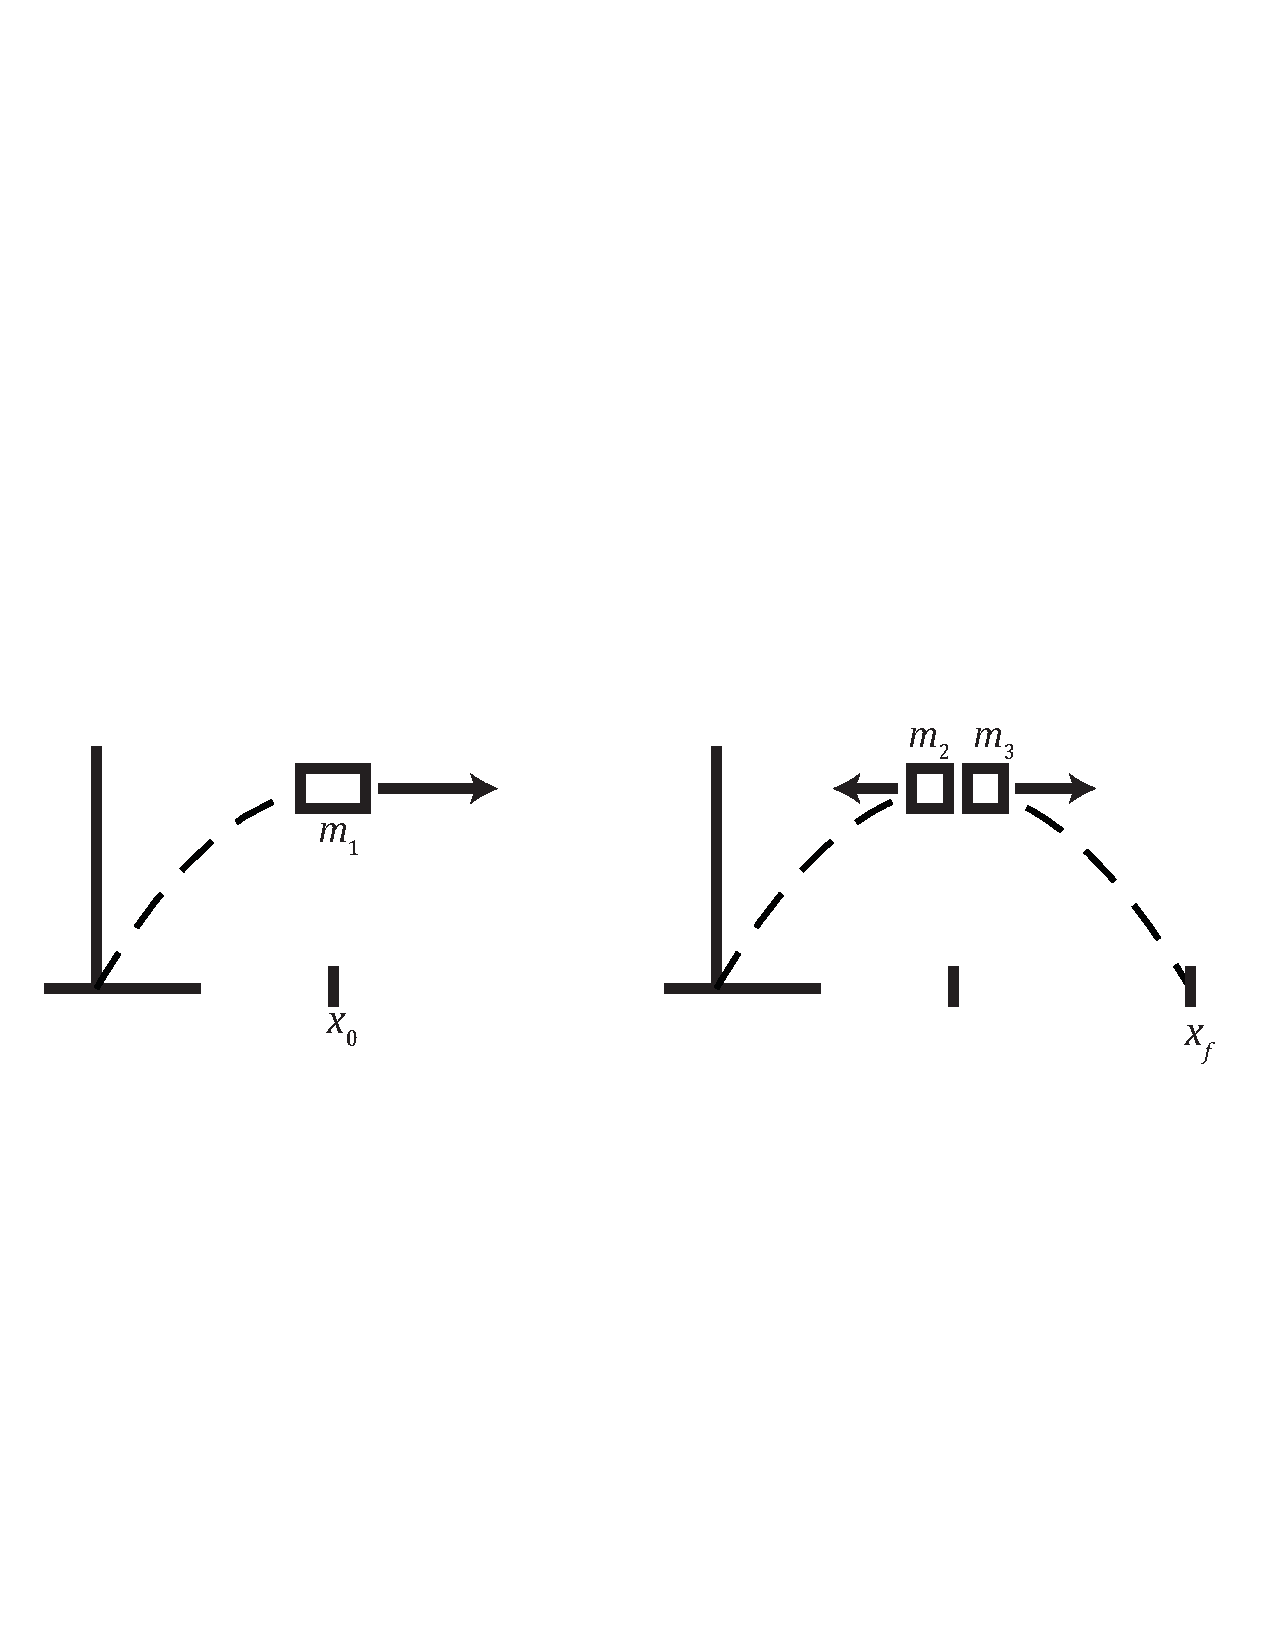
\includegraphics[width=0.5\textwidth]{ps_04_1}\end{center}
%\begin{enumerate}[a)]
%  \item What is the velocity of the projectile at the top of its flight just before the collision?
%  \item What is the velocity of the smaller piece just after the collision?
%  \item What is the velocity of the larger piece just after the collision?
%  \item
  How far away, $x_f$, from the original launching point does the larger piece land?
%\end{enumerate}
\section*{Problem 4: K\&K 3.6}
  A light plane weighing 2500 lb makes an emergency landing on a short runway. With its engine off, it lands on the runway at a speed of 120 ft / sec. A hook on the plane snags a cable attached to a 250 lb sandbag and drags the sandbag along. If the coefficient of friction between the sandbag and the runway is $\mu_k = 0.4$, and if the plane's brakes give an additional retarding force of magnitude 300 lb, how far does the plane go before it comes to a stop?
\section*{Problem 5: K\&K 3.7}
  A system is composed of two blocks 1 and 2 of masses $m_1$ and $m_2$ respectively that are connected by a massless spring with spring constant $k$. The blocks slide on a frictionless plane. The unstretched length of the spring is $l$. Initially the block 2 is held so that the spring is compresses to a length $l / 2$ and block 1 is pushed up against a wall. At $t = 0$ block 2 is released. Find the motion of the center of mass of the system as a function of time.
\section*{Problem 6: K\&K 3.11}
  Material is blown into cart A from cart B at a rate of $b$ kilograms per second. The material leaves the chute vertically downward, so that it has the same horizontal velocity, $u$ as cart B. At the moment of interest, cart A has mass $m_A$ and velocity $v$.
  \begin{center}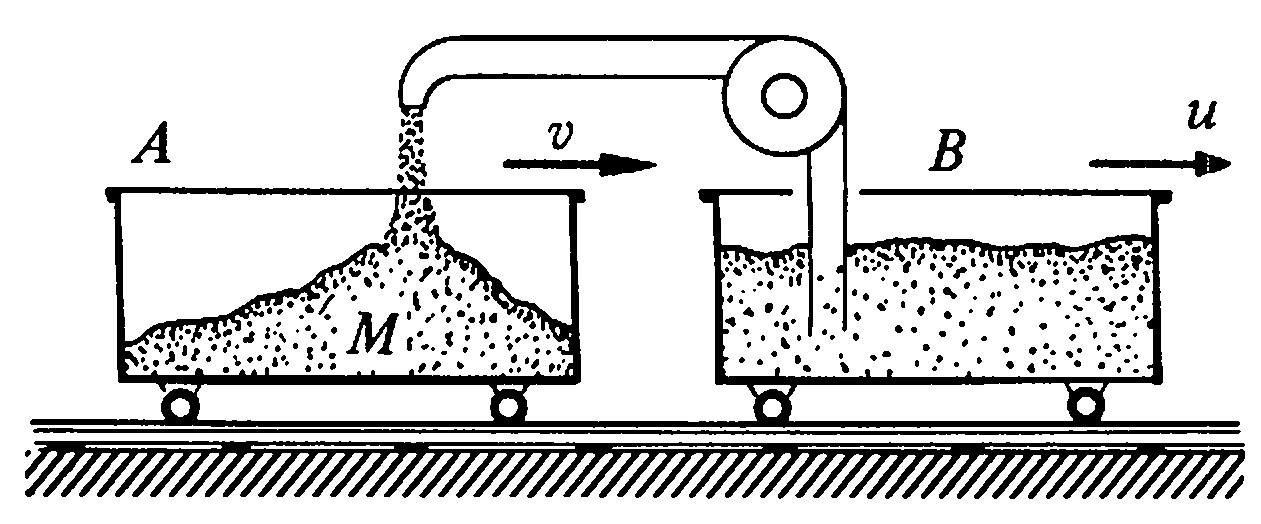
\includegraphics[width=0.5\textwidth]{ps_04_2}\end{center}
  \begin{enumerate}
    \item Define the objects that will constitute your system.
    \item Based on momentum diagrams, derive a differential equation for the velocity $v$.
    \item In particular find an expression for the rate of change of velocity, the instantaneous acceleration, $d v / d t$.
    \item Integrate this equation to find the velocity has a function of time.
  \end{enumerate}
\section*{Problem 7: K\&K 3.12}
  A sand-spraying locomotive sprays sand horizontally into a freight car. The locomotive and freight car are not attached. The engineer in the locomotive maintains his speed so that the distance to the freight car is constant. The sand is transferred at a rate $d m / d t = 10$ kg/s with a velocity $u = 5$ m/s relative to the locomotive. The car starts from rest with an initial mass of 2000 kg. Find its speed after 100 s.
  \begin{center}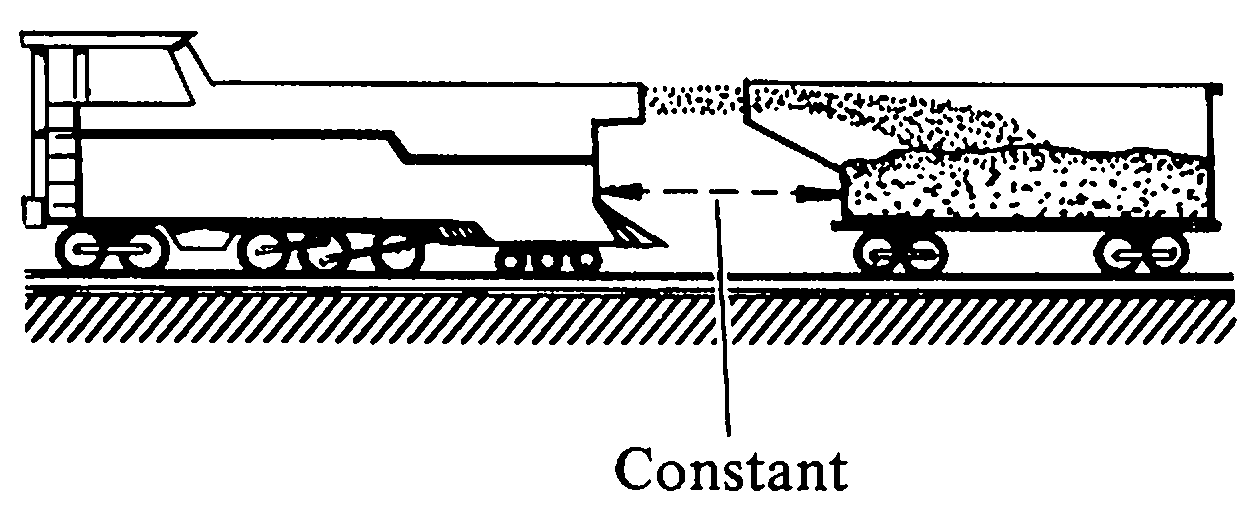
\includegraphics[width=0.5\textwidth]{ps_04_3}\end{center}
\end{document}
